\documentclass[11 pt]{article}

\usepackage{natbib}
\usepackage[nottoc]{tocbibind}

\usepackage[utf8]{inputenc}
\usepackage[T1]{fontenc}
\usepackage[french]{babel}

\usepackage{amsmath}
\usepackage{empheq}
\usepackage{tikz}
\usepackage{tikz-qtree}
\usepackage{listings}
\usepackage{graphicx}
\usepackage{algorithm2e}
\usepackage[left=2cm,right=2cm,top=1.5cm,bottom=1.5cm]{geometry}
\usepackage[toc,page]{appendix}
\usepackage{hyperref}
\hypersetup{
  colorlinks,
  citecolor=black,
  filecolor=black,
  linkcolor=blue,
  urlcolor=blue
}
\usepackage{appendix}
\usepackage{enumitem}           % modified itemize
\usepackage{float}

\title{Projet Transboost}
\author{Luc Blassel, Romain Gautron, Xue Bai, Yifei Fan, Xuefan Xu}

\begin{document}
\maketitle

\tableofcontents
\newpage

\section{Context}
% \paragraph{}L’apprentissage supervisé  classique nécessite un grand nombre de données étiquetées, et dans certains cas une période de temps très importante pour pouvoir établir des modèles fiables. Ceci n’est pas toujours possible dans le monde réel, parfois il n’est simplement pas possible de collecter assez de données pour entraîner nos modèles ou alors le temps necessaire pour l’entrainement du modèle est beaucoup trop long pour que ce soit utilisable en pratique avec des ressources conventionnelles. L’apprentissage par transfert peut nous aider à résoudre ce type de problèmes.
\paragraph{}Classical supervised learning requires a large amount of labeled data and, in certain cases, a very long amount of time to ba able to train reliable models. This is not always possible in a `real world' setting, it could be that it is not possible to obtain sufficient data to train models or that the required time for training is so long that it becomes practically unfeasible with conventional resources. Transfer learning can help us solve this type of problem. 

% \paragraph{}L’apprentissage par transfert nous permet de transférer des connaissances apprises depuis domaine source avec idéalement une grande quantité de données étiquetées de bonne qualité, vers un domaine cible. Cette approche permet de réutiliser des portions d’un modèle préalablement entrainé dans notre nouveau modèle. L'avantage est double : économie en temps de calcul et utilisation d'une quantité limitée de données en réinvestissant de l'information provenant d'une autre tâche. Cette méthode est considérée comme le prochain moteur de succès de l’apprentissage automatique après l’apprentissage supervisé.
\paragraph{}Transfer learning allows for a transfer of acquired knowledge from a source domain, ideally with a large amount of well labeled data, towards a target domain. With this approach, portions of a pre-trained model can be reused in a new model. The advantage is two-fold: training times are shortened and the amount of training data needed is smaller. This method is considered by some as the next motor of progress in automatic learning after supervised learning. 

% \paragraph{}La méthode TransBoost \cite{transboost}, introduite par Antoine Cornuéjols et ses collègues propose une implémentation de l’apprentissage par transfert différente de l'usage. Quand l’approche “classique” de l’apprentissage par transfert adapte l'hypothèse développée sur le domaine source au domaine cible, TransBoost en prend le contre-pied. En effet dans cette dernière on apprend l'hypothèse sur le domaine source et on projette ensuite les points du domaine cible sur le domaine source pour utiliser directement l'hypothèse source sur les points projetés.
\paragraph{}The TransBoost method \cite{transboost}, proposed by Antoine Cornuéjols et al., outlines a different approach than "classical" transfer learning. Where the latter adapts the hypothesis learned on the source space, to the target space, TransBoost does the opposite. The hypothesis is learned on the source space and the data points from the target space are projected in the source space to make use of the source hypothesis without the need to relearn it.

% \paragraph{}Ainsi, on n'apprend pas de nouvelles frontière entre les points, on injecte plutôt les points des bons côtés des frontières source. La projection des points du domaine cible sur le domaine source se fait dans le cadre d'un algorithme de boosting, qui grâce à plusieurs projecteurs faibles, permet d’obtenir un projecteur fort. Ce dernier permet alors d’utiliser l'hypothèse source pour classifier les points du domaine cible. La différence d'approche entre apprentissage par transfert "usuel" et Transboost est illustrée sur le schéma ~\ref{figDiff}.
\paragraph{} This way no new frontiers between points are learned, the target points are correctly projected at the right location in the source domain. This projection is done within a boosting algorithm, allowing for the building of a strong projector by combining several weak projectors. This difference in approaching the issue can be seen in Figure \ref{figDiff}. 


% \paragraph{}L'approche Transboost a d’abord été testée sur la classification des séries temporelles incomplètes et à été un franc succès en ayant de bien meilleures performances que d’autres approches du même problème. Cependant, la classification d’images étant le mètre étalon en ce moment, le but de ce projet est d’adapter la méthode TransBoost à la classification d’images en utilisant des réseaux de convolution profonds (deep CNN). Ce travail ne présente que la classification binaire d'images.
\paragraph{}The TransBoost method has been tested on classification of incomplete time series data with real success, outperforming other methods used for this problem. However, image classification being the standard measure right now, this project intends to adapt the TransBoost method toimage classification unsing deep convolutionnal neural networks (CNN). In this project only binary classification is tried.  

\begin{figure}[H]
  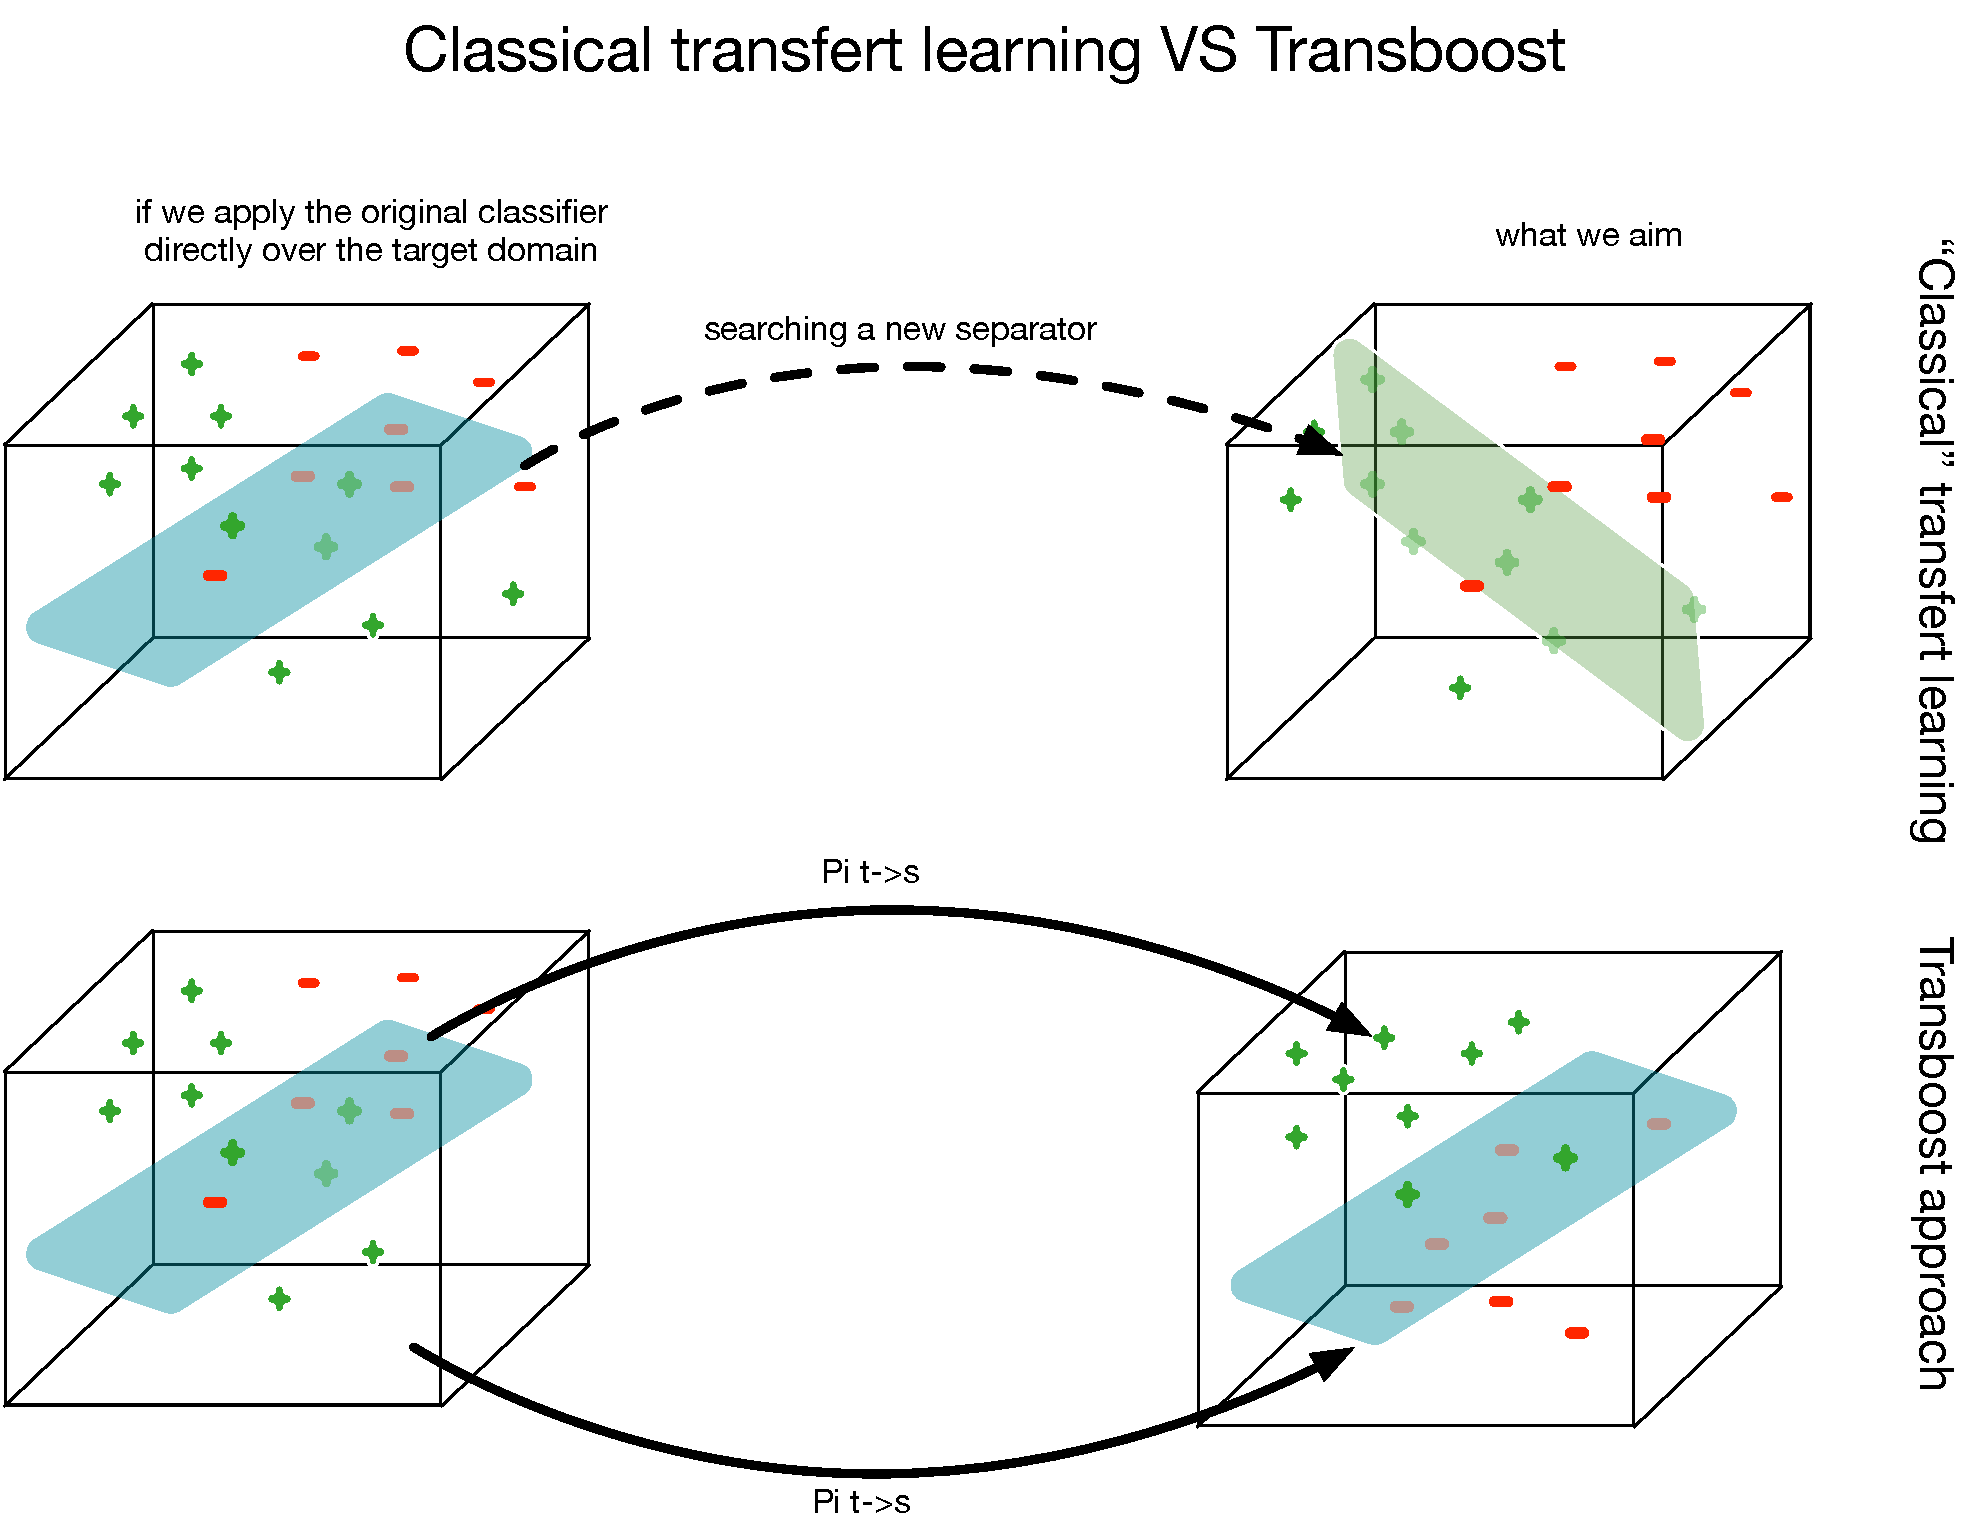
\includegraphics[width=\textwidth]{fig2.pdf}
  % \caption{Différences entre l'approche classique et l'approche TransBoost}
  \caption{Differences between "classical" transfer learning and the TransBoost method}
  \label{figDiff}
\end{figure}

\section{Transboost pour la classification d'images : principe}

\paragraph{}L’application de la méthode TransBoost à la classification d’images oblige à se poser plusieurs questions. D’une part la très grande dimensionnalité des images force a utiliser des méthodes très lourdes telles que les réseaux de convolution profonds, c'est donc un défi en terme de puissance de calcul. D’autre part comment réaliser la projection des points du domaine cible dans le cas d'images ?

% D'autre part, il existe dans les librairies de machine learning telles que \texttt{Tensor Flow} des réseaux pré-entraînés, mais quel modèle choisir, pourquoi?
% \paragraph{}Contrairement a l’apprentissage par transfert “classique”  il ne s’agit pas ici d’adapter l'hypothèse source au domaine cible, comme ce que l’on peut voir sur la première partie du schéma. Il faut donc projeter les points du domaine cible sur le domaine source avec une bonne précision pour que la séparatrice du classificateur source puisse différencier les images du domaine cible.\\

% \paragraph{} Le choix a été fait de modifier les premières couches du réseau "source" pour classifier les images du domaine cible. Ainsi, les premières couches du réseau existant se chargeront de trouver les bons descripteurs de faible niveau pour que la nouvelle tâche puisse être réalisée. Cependant il faudra trouver les meilleurs hyper-paramètres de ces projecteurs (voir infra).
\paragraph{} The choice has been made, to modify the lower layers of the source network to classify target images. Therefore, the lower layers of the existing network will find the right low-level descriptors so that the new task can be done. However hyper-parameter optimization will have to be done.

% \paragraph{} On aurait pu également construire une réseau externe qui se charge d'être le projecteur des images et qui arrive en entrée du réseau "source". Celui-ci aurait eu en entrée des images et en sortie également des images (visualisation intéressante). A noter que cette option aurait été plus lourde en calculs (backpropagation supplémentaire) et ne sera pas explorée ici.
\paragraph{} We could also have implemented a separate "projector" network that would take the source domain images and transform them in projected images. Howver, even though potentially visually interesting, it would have required larger computing power (more back-propagation) and was not implemented.

\pagebreak

\begin{samepage}
La construction d'un projecteur s'effectue comme suit : \medskip
  \begin{itemize}
    \item On obtient un réseau convolutionnel très performant sur une classification binaire source et aussi bon que le hasard pour une classification binaire cible. Les modèles pré-entraînés disponibles ont souvent un grand nombre de classes de sortie. Il est nécessaire de changer la couche de sortie du réseau et de l’entraîner pour l’ajuster à notre domaine source binaire.
    \nopagebreak
    \item On gèle la partie supérieur dudit réseau en laissant les premières couches entraînables.
    \nopagebreak
    \item On ré-entraîne ledit modèle partiellement gelé pour obtenir un projecteur en visant une valeur de métrique seuil pour arrêt. Nous choisissons la précision comme métrique, celle-ci étant parlante et pertinente dans le cas de datasets équilibrés en classes.
  \end{itemize}
\end{samepage}

On construit itérativement un ensemble de projecteurs faibles spécialisés sur les erreurs des précédents selon l'algorithme Adaboost \cite{boosting}. Notre hypothèse finale sur le domaine cible sera une combinaison de ces projecteurs faibles.

\section{Application}

Dans toute cette section, la figure~\ref{figRes} illustrera les propos.

\begin{figure}[H]
  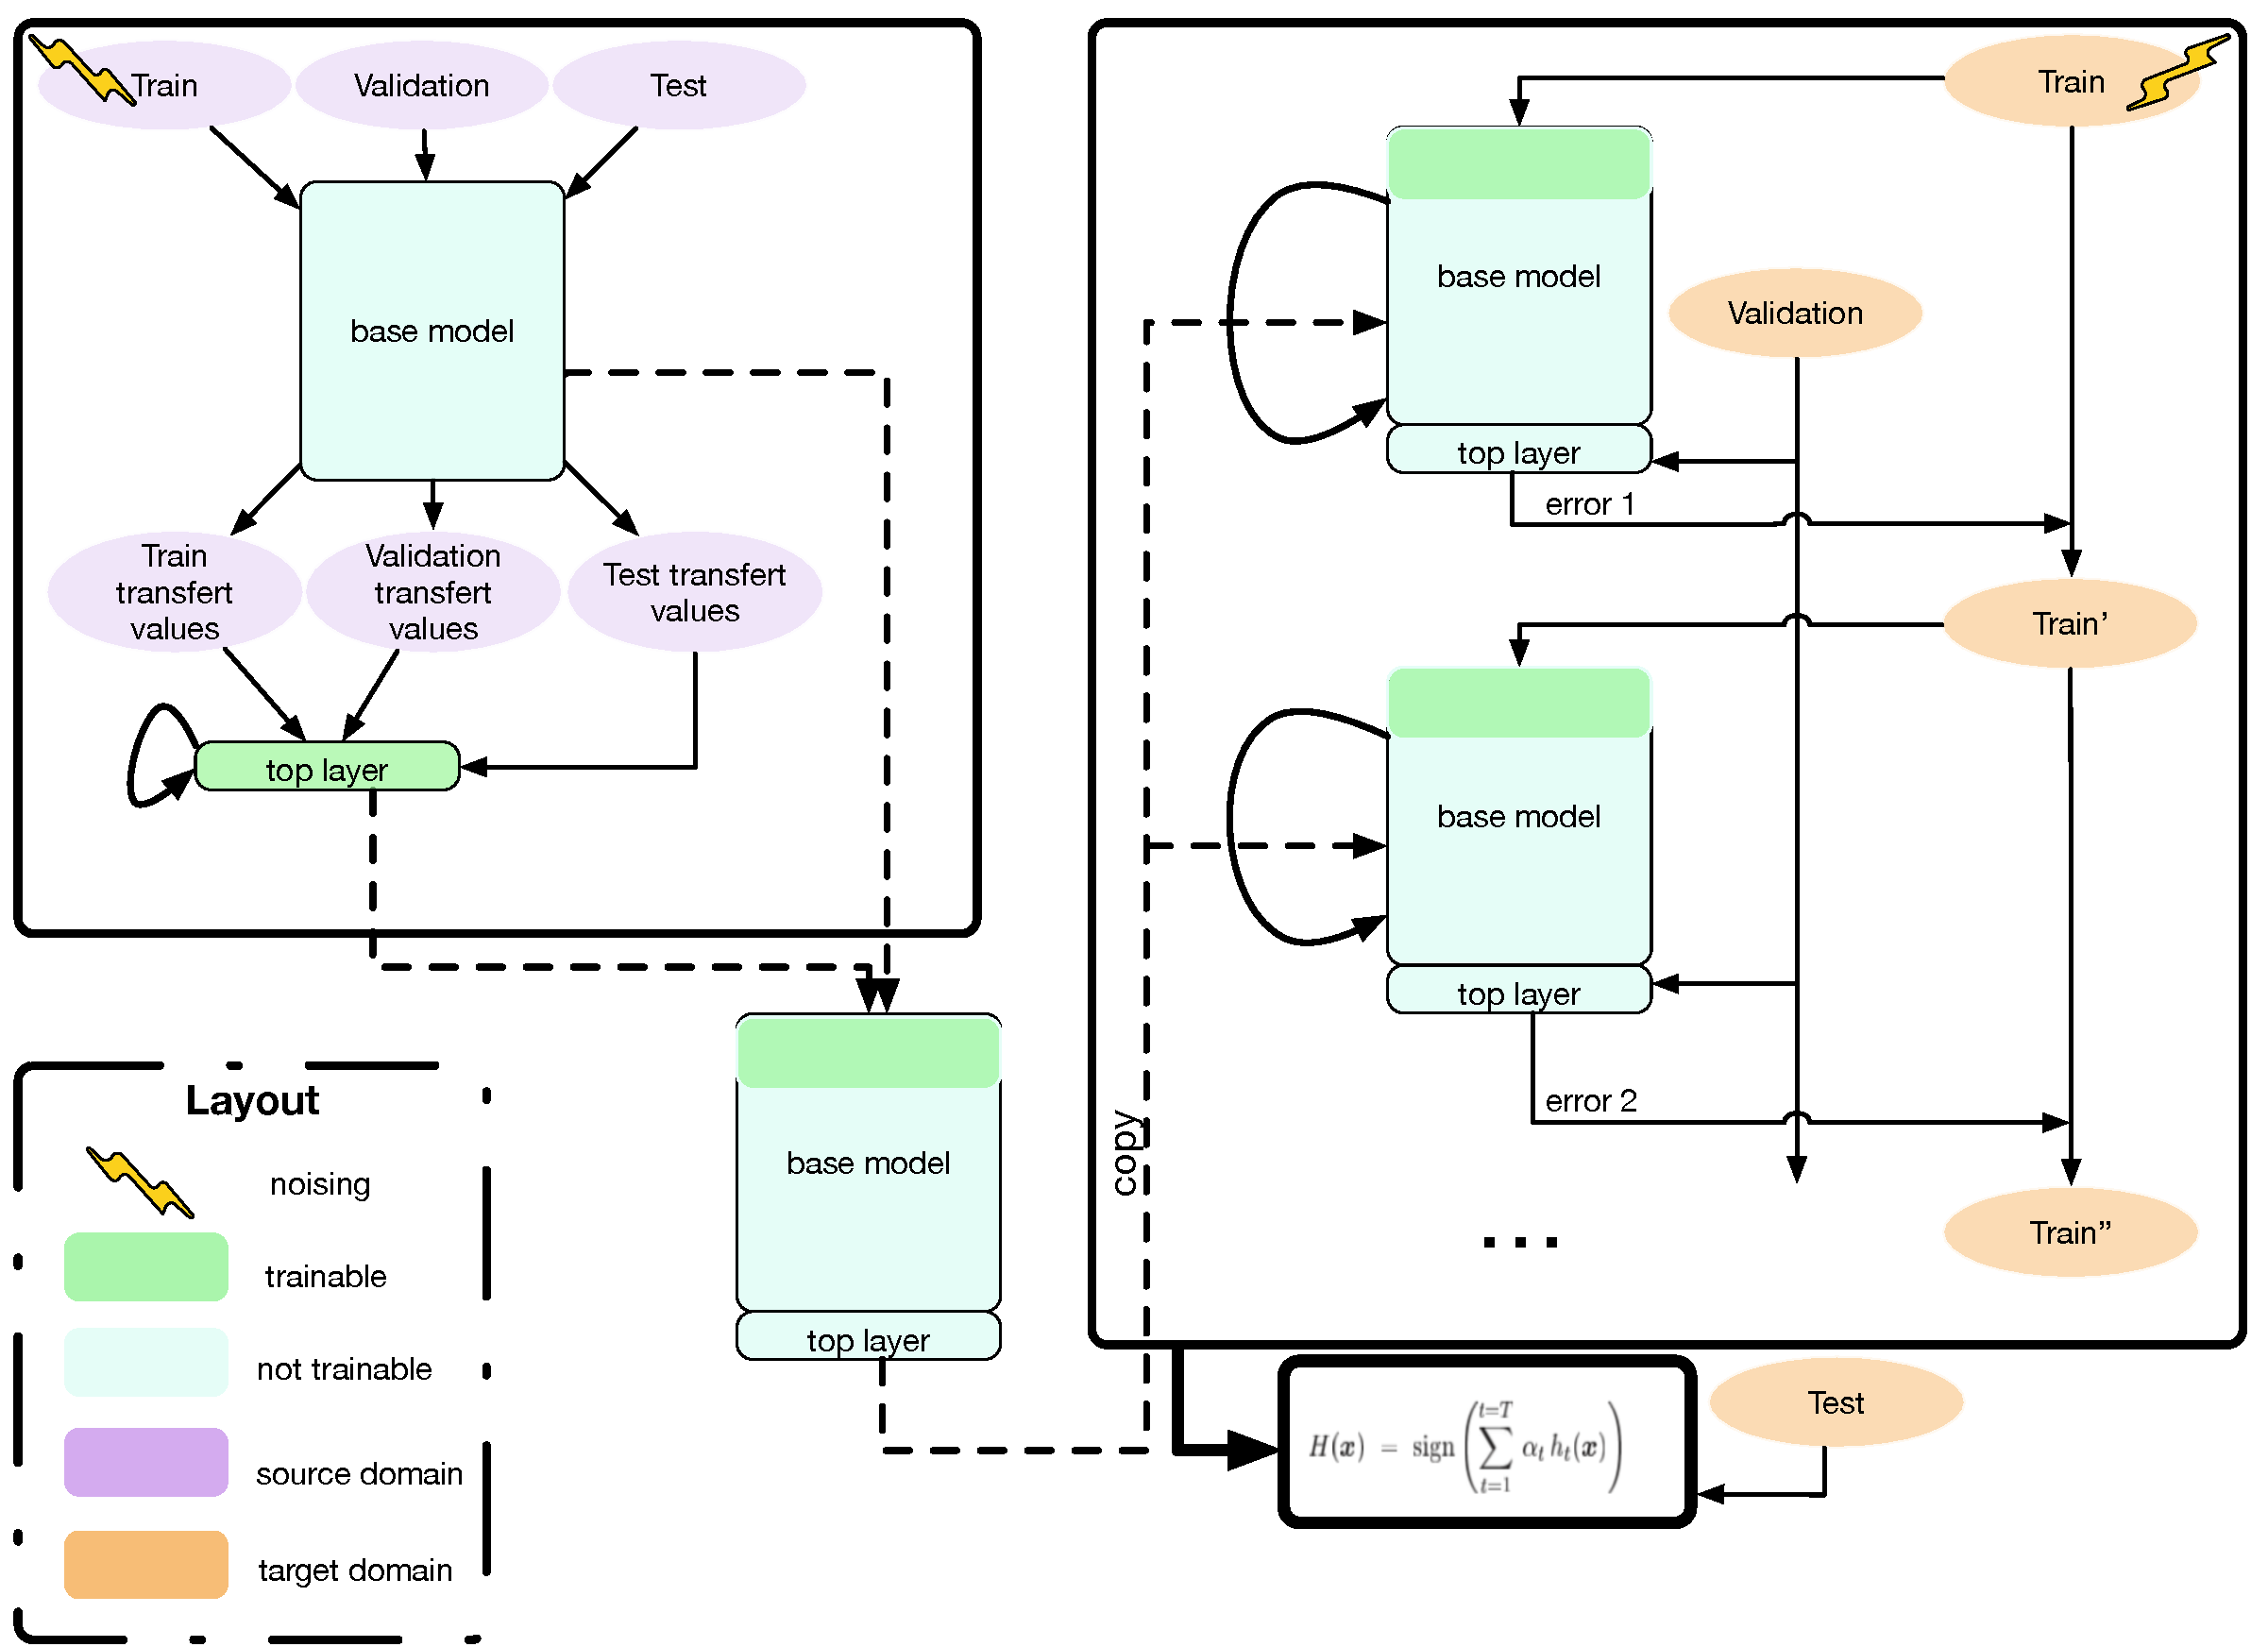
\includegraphics[width=\textwidth]{fig1.pdf}
  \caption{Déroulement de la méthode TransBoost dans le cadre de ce projet}
  \label{figRes}
\end{figure}

\subsection{Présentation des données}
\paragraph{}Nous avons choisis le data set CIFAR-10 composé d’images RGB 32x32. Celui-ci est composé de 60000 images se ventilant en 10 classes (avion,automobile,oiseau,chat,cerf,chien,grenouille,cheval,bateau,camion). Les motivations pour ce choix sont :\\ \medskip
\begin{itemize}
  \item qu’il s’agit d’un dataset de référence usuel dans le milieu
  \item que la faible de taille des images limite le volume des données à manipuler
  \item le faible nombre de classes permet néanmoins de constituer des couples plus ou moins ardus (avion/chat vs chien/chat)
\end{itemize}

\paragraph{}Les données sont déjà reparties en 3 ensembles : entraînement, validation et test. Pour pallier au faible nombre des données dans la base d’entraînement on introduira du bruit dans celles-ci pour éviter tout sur-apprentissage. Ce bruit consiste en des rotations, zooms, déformations aléatoires. Attention, aucun bruitage n’est appliqué aux ensemble de validation et de test. En effet, on veut ceux-ci les plus représentatifs possible des images “réelles” pour éprouver le modèle.

\paragraph{}Pour constituer les ensembles source et cible, il s’agit dans les faits de simple paramètres d’entrées qui permettent de changer les classes de manière aisée (exemple : classes\_source = ['dog','truck'], classes\_target = ['deer','horse']). A noter que le bruitage des sets d’entraînement est appliqué pour les deux domaines.



\subsection{Construction d'un classifieur binaire fort sur le domaine source}
\paragraph{}Afin de pouvoir mettre en application l’idée du TransBoost, nous devons tout d’abord obtenir un classifieur binaire fort sur une tâche et aussi bon que le hasard sur une seconde. Pour cela, nous devons d’abord choisir quel sera notre modèle de base. On entend par modèle de base un réseau profond déjà entraîné et sans les dernières couches (couches connectées et softmax). \texttt{Keras} offre de nombreuses possibilités de modèles (voir \href{https://keras.io/applications/}{ce lien}). Le choix s’est porté sur le modèle Xception, d’une part pour la qualité des valeurs de transferts qu’il produit et d’autre part pour le temps qu’il faut pour générer ces valeurs de transfert. On appelle valeurs de transfert les valeurs des fonctions d’activation de la dernière couche du modèle de base pour un ensemble d’images.

\paragraph{}Par soucis de parcimonie en temps de calcul, on fait passer l’ensemble des sets d’images dans le modèle de base une seule fois. On génère ainsi les valeurs de transfert qui serviront à l’entraînement de la dernière couche. \\
L’architecture de la dernière couche (plus exactement du dernier bloc) est :\\ \medskip
\begin{samepage}
  \begin{itemize}
    \item une couche entièrement connectée de taille 1024, activation “relu”
    \nopagebreak
    \item un dropout à 50 \%
    \nopagebreak
    \item une couche entièrement connectée de taille 512, activation “relu”
    \nopagebreak
    \item un dropout à 50 \%
    \nopagebreak
    \item un couche de taille 1, activation “sigmoïd”
  \end{itemize}
\end{samepage}

\medskip

\paragraph{}Le choix de l'architecture s’est fait de manière empirique.\\

Comme pour le bruitage des images, le dropout est ici pour prévenir le surapprentissage compte tenu du faible nombre d’images présentées.
Une fois la dernière couche entraînée et répondant aux caractéristiques désirées, on assemble le modèle de base et ladite dernière couche en un modèle complet.


\subsection{Mise en pratique du TransBoost}
\paragraph{}Une fois que nous avons constitué notre classifieur fort, il faut voir la suite comme l’application classique d’Adaboost. La seule nuance est que, au lieu de repartir d’un classifieur “from scratch” on va cette fois partir d’un classifieur partiellement entraîné pour constituer notre projecteur faible.

\paragraph{}On cherche, non pas comme dans le transfert learning classique avec les CNN à réapprendre une nouvelle séparatrice linéaire en entraînant la dernière couche pour une nouvelle tâche. On cherche à faire rentrer pour la nouvelle tâche les points des bons cotés de la séparatrice pour la tâche précédente en cherchant des descripteurs de faibles niveau correspondants (i.e. en ré-entraînant les premiers blocs du réseaux de neurones profond) pour que cela soit réalisé.

\paragraph{}Pour ce faire,  on prend le modèle que nous avions à l’étape précédente, on dégèle les premières couches du modèle de base et on gèle tout le reste. A ce stade deux approches sont possibles : soit réinitialiser les poids des couches dégelées soit conserver les poids. Il se peut qu’en réinitialisant le poids de ces couches avec des descripteurs de faible niveau ne permette pas à l’algorithme de converger sur si peu de données. La réponse viendra des expérimentations. Dans les deux cas, le modèle résultant de l’étape citée servira de classifieur à entraîner lors des étapes de boosting.\\

Trois paramètres importants sont à chercher selon un compromis performances/coût calculatoire :\\ \medskip
\begin{itemize}
  \item la force des classifieurs (seuil de précision) à chaque étape de boosting
  \item le nombre de blocs convolutifs à entraîner
  \item le nombre de projecteurs faibles entraînés
\end{itemize}

\paragraph{}La suite est celle de l’algorithme Adaboost (voir ~\ref{ada}). A noter que l’erreur totale du modèle est mesurée sur le set de validation. Par contre le modèle est bien entraîné sur le set d’entraînement pondéré, et la pondération des points basée sur les prédictions faites sur ce même set d’entraînement.\\

A chaque étape, l’entraînement d’un projecteur s’arrête lorsqu’un seuil de précision est atteint (avec une limite d’un grand nombre d’epochs).

\pagebreak

\begin{algorithm}[H]
  \SetAlCapSkip{10ex}
  \SetKwInOut{Input}{input}\SetKwInOut{Output}{output}
  \SetKw{Init}{Initialisation:}
  \Input{$\mathcal{X_S}\rightarrow\mathcal{Y_S}$ :  l'hypothese source\\
          $\mathcal{S_T = \{(X_I^T,Y_I^T)\}}_{1\leq i\leq m}$ : l'ensemble d'entrainement cible}
  \Init{} de la distribution sur le jeu d'entrainement:$D_1(i)=1/m\ for\ i=1,\cdots,m$\;
  \For{$n=1,\cdots,N$}{
    Trouver une projection $\pi_i:\mathcal{X_T\rightarrow X_S}$ tq. $h_S(\pi_i(.))$ soit meilleure que le hasard sur $D_n(\mathcal{S_T})$\;
    Soit $\epsilon_n$ le taux d'erreur de $h_S(\pi_i(.))$ sur $D_n(\mathcal{S_T})$: $\epsilon_n = P_{i~D_n}[h_S(\pi_n(x_i))\neq y_i]$(avec $\epsilon_n<0.5$)\;{}
    Calculer $\alpha_i=\frac{1}{2}log_2(\frac{1-\epsilon_i}{\epsilon_i})$\;
    Mettre a jour: \For{$i=1,\cdots,m$}{
        \begin{equation*}
          \begin{split}
            D_{n+1}(i) & = \frac{D_n(i)}{Z_n}\times\begin{cases}
              e^{-\alpha_n}\ si\ h_{\mathcal{S}}(\pi_n(x_i^{\mathcal{T}}))=y_i^{\mathcal{T}} \\
              e^{\alpha_n}\ si\ h_{\mathcal{S}}(\pi_n(x_i^{\mathcal{T}}))\neq y_i^{\mathcal{T}}
            \end{cases}\\
            & = \frac{D_n(i)exp(-\alpha_n y_i^{(\mathcal{T})}h_{\mathcal{S}}(\pi_n(x^{(\mathcal{T})})))}{Z_n}
          \end{split}
        \end{equation*}
        Ou $Z_n$ est un facteur de normalisation tq. $D_{n+1}$ soit une distribution de $\mathcal{S_T}$\;
    }
  }
  \Output{L'hypothese finale $H_{\mathcal{T}}:\mathcal{X_T \rightarrow Y_T}$:\\
            $ H_{\mathcal{T}}(x_{\mathcal{T}})=signe\{\sum\limits_{n=1}^N \alpha_n h_{\mathcal{S}}(\pi_n(x^{\mathcal{T}}))\}$}

  \caption{Algorithme Transboost}
  \label{ada}
\end{algorithm}

\subsection{Difficultés rencontrées}
\paragraph{}Nous avons fait la décision initiale de travailler dans un environnement purement \texttt{Tensor Flow}, puisque le modèle que nous avions choisi était disponible dans cette librairie. Cependant dès qu’il a été temps de modifier la structure du modèle (pour avoir une couche de sortie binaire par exemple) ou qu’il a fallu geler l'entraînement de certaines couches l’utilisation de \texttt{Tensor Flow} est devenue très compliquée. En effet l’objet du modèle était introuvable et il fallait modifier un graphe ce qui nous a posé beaucoup de problèmes. C’est pour cela que nous avons décidé d’utiliser la librairie \texttt{Keras} qui fonctionne comme surcouche de \texttt{Tensor Flow} ce qui nous a permis d’utiliser les modèles disponible dans \texttt{Tensor Flow} mais en ayant des outils et une syntaxe plus claire et plus simple d’utilisation, permettant des temps de développement beaucoup plus courts.

\paragraph{}Nous avons aussi rencontré beaucoup de problèmes de ressources machine, puisque les machines physiques et virtuelles auxquelles nous avions accès présentaient des performances limitées. Ceci a engendré des temps d'exécution se comptant en dizaine d’heures et même en jours dans certains cas et aboutissant souvent a des erreurs de mémoire. Il est donc nécessaire d’avoir accès à une machine performante qui nous permettra débugger le programme et le perfectionner sans attendre des périodes très longues.

\section{Comparaisons critiques portant sur la méthode transboost}
\subsection{Projecteurs faibles vs. projecteurs forts}
\paragraph{}On veut comparer l’approche TransBoost avec faisant varier la force des projecteurs aux extrêmes. Si l’on obtient des performance supérieures avec un seul projecteur fort (i.e. les premiers groupes de couches convolutives entraînées aux maximum) alors on ne peut pas montrer un intérêt de travailler avec une multitudes de projecteurs faibles en boosting dans ce cadre précis.

\subsection{Projecteurs vs. nouveaux classifieurs}
\paragraph{}Comme on le voit, la méthode du TransBoost appliquée avec le modèle complet (base et dernier bloc) est très gourmande en temps et en espace. En effet, après avoir entraîné un grand nombre de classifieurs il faut également stocker tous ceux-ci à fin de pouvoir réaliser les classification de nouveau points selon l’hypothèse finale. En fait, on peut être plus économe en espace. En effet, il suffit de la connaissance pour reconstruire tous les modèles issus du boosting :\\ \medskip
\begin{itemize}
  \item du modèle complet non modifié
  \item uniquement pour chaque étape de boosting du poids des couches modifiées
\end{itemize}
\paragraph{}On souhaite mettre en compétitions deux approches : le TransBoost et une méthode de boosting classique.

\paragraph{}On peut atteindre un seuil de précision relativement bas à chaque étape ( de l’ordre de 0.7) simplement à l’aide d’un petit réseau convolutif initialisé (quelques blocs). Bien qu’avec l’économie en espace citée précédemment il n’y ait pas beaucoup de différence, l’économie en temps de calcul est bien là. En effet pour chaque prédiction à faire, le passage dans le petit CNN suffit. Tandis qu’à chaque étape avec le modèle de base augmenté du dernier bloc il faille calculer les activations dans toute la partie supérieure gelée du réseau avant de "backpropager" l’erreur.



\section{Resultats}
\subsection{Construction du classifieur binaire}
\paragraph{}Dans les faits, pour la base d’apprentissage “chien/camion”, l’algorithme arrive à 98.9\% de précision sur le set de test en seulement 2 epochs. D’un autre côté ce même modèle entraîné sur le dataset précédent a un précision de 50\% en prédiction sur le dataset “deer/horse”, ce qui répond bien à ce que l’on recherchait.

\subsection{Boosting classique sur petit CNN}
\paragraph{}Avec un petit nombre de projecteurs (12) et un petit CNN (3 blocs de convolution) on arrive à une précision de 76.8\% en test sur le dataset “horse/deer”. Expérience à renouveler avec un 100 projecteurs dès qu’on aura la puissance de calcul ad hoc.

\section{Experimentations a venir}
\subsection{Comportement de l'algorithme Transboost}
\subsubsection{Influence des domaines source et cible}
\paragraph{}Peut t-on partir d’un domaine source simple (ex : “dog/truck”) pour aller vers un domaine cible plus compliqué (ex:”deer/horse”) ?

\paragraph{}Bien sur dans les temps venant il faudra tester les critiques soulevées plus haut, en comparant les performances des projecteurs faibles contre un projecteur fort, et la performance de ces projecteurs par rapport à celle d'un classifieur nouvellement entraîné.


\subsubsection{Influence des hyper-paramètres: recherche d'un optimum précision/coût calculatoire}
\paragraph{Influence de la force des projecteurs}
\paragraph{Influence du nombre de projecteurs}
\paragraph{Influence du nombre de blocs entraînés}
Dans l’idéal on veut en modifier le moins possible pour atteindre au plus vite le seuil de précision

\subsection{Comparaisons critiques de l'algorithme Transboost}
\subsubsection{Projecteurs faibles vs. projecteurs forts}
\subsubsection{Projecteurs vs. nouveaux classifieurs}
\paragraph{}

\bigskip
\nocite{*}
\bibliographystyle{plain}
\bibliography{biblio.bib}

\pagebreak
\begin{appendices}
  \section{Code}
    \href{https://gitlab.com/zlanderous/transboost}{Code sur gitlab.}

  \section{Schéma du programme}
  \begin{figure}[h]
    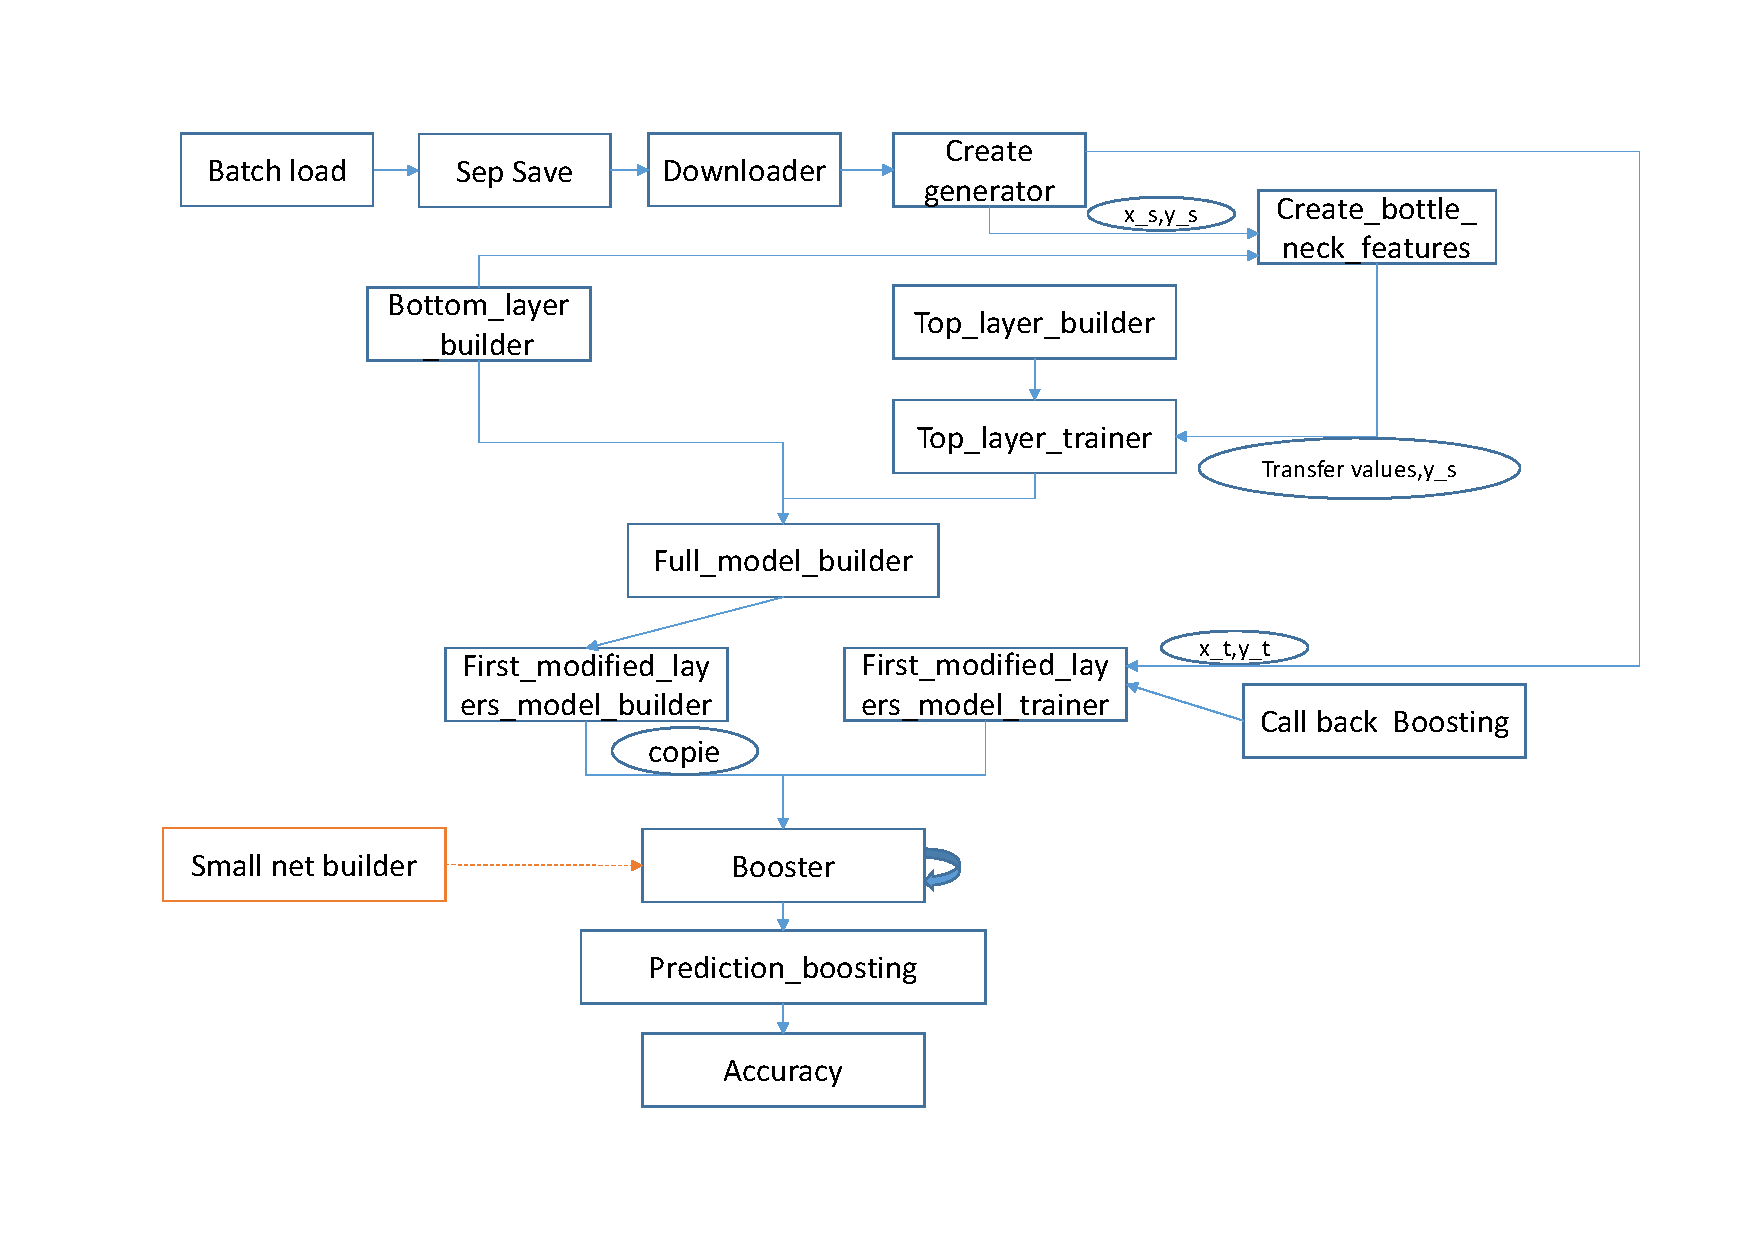
\includegraphics[width=\textwidth]{figTot.pdf}
    \caption{schema du programme}
    \label{figTot}
  \end{figure}
  \paragraph{}Descriptif des fonctions:\\

  \begin{description}
    \item[Batch\_loader:] Prend les images d'un batch de CIFAR-10 et les enregistre dans un dictionnaire avec comme clé la classe de l'image.
    \item[Sep\_saver:] Parcourt le dictionnaire et enregistre les images de chaque classe dans un dossier correspondant.
    \item[Downloader:] Télécharge les batches de CIFAR-10 et exécute les deux fonctions précédentes pour chaque batch d'entrainement, de test et de validation.
    \item[Create\_generator:]
    \item[Bottom\_layer\_builder:] Charge et construit le modèle sans derniere couche (Xception dans ce cas).
    \item[Create\_bottleneck\_features:] Calcule les valeurs de transfert pour chaque image des jeux d'entrainement, de test et de validation passant par le modèle issu de la fonction précédente.
    \item[Top\_layer\_builder:] Construit la couche de sortie binaire.
    \item[Top\_layer\_trainer:] Entraine la dernière couche avec les valeurs de transfert.
    \item[Full\_model\_builder:] Assemble le modèle sans derniere couche et la dernière couche nouvellement entraînée.
    \item[First\_modified\_layers\_model\_builder:] Gèle les poids des $n$ dernières couches pour effectuer le boosting.
    \item[First\_modified\_layers\_model\_trainer:] Entraine le modèle partiellement gelé sur le jeu d'entrainement.
    \item[Callback\_boosting:] est appelé à chaque epoch de l'entrainement du modèle et si la précision est supérieure à un seuil $\alpha$ arrête l'entraînement.
    \item[Booster:] Applique l'algorithme adaboost au réseau. chaque modèle entraîne faisant office de projecteur faible est construit puis entraîne en appelant les deux fonctions précédentes $n$ fois.
    \item[Prediction\_boosting:] Effectue un e prédiction sur la classe de l'image présentée en prenant en compte les modèles entraînés dans la fonction précédente.
    \item[Accuracy:] Évalue la précision des prédictions.
  \end{description}
\end{appendices}

\end{document}
